Following \cite{Hirsch}, the DGMPM discretization of linear advection problems are now written in a finite difference sense. The scheme equations thus obtained are the starting points for von Neumann linear stability analyses. First, the one-dimensional problem is considered and scheme equations based on the DGMPM space discratization, combined to both forward Euler and \textit{second-order Runge Kutta (RK2)} explicit time discretizations, are derived. Second, the two-dimensional scheme equation is written by using the DGMPM space discretizattion along with the explici forward Euler time discretizattion only.

\subsection{One-dimensional DGMPM scheme equations}
\subsubsection*{Model equation - Space discretization}
We consider the scalar linear advection equation for an arbitrary quantity $q=\rho \bar{q}$ moving at the constant speed $a \in \Rbb^{+*}$ in a homogeneous one-dimensional medium of length $l$:
\begin{equation}
\drond{\bar{q}}{t} + a\drond{\bar{q}}{X} = 0 \label{eq:scalar_advection}
\end{equation}
The specific flux function is $\bar{\Fc} = a\bar{q}$ and equation \eqref{eq:scalar_advection} is discretized with the discontinuous Galerkin material point method. Thus, it is assumed that the medium has been divided with $N_p$ material points arbitrarily distributed in $E$ two-nodes elements of constant length $\Delta X$ (figure~\ref{fig:1Dmesh}). The grid mesh is such that at least one particle lies in every cell during the computation in order to ensure that there is no hole in the bar. Moreover, periodic boundary conditions are considered to simplify the analysis.
\begin{figure}[h!]
  \centering
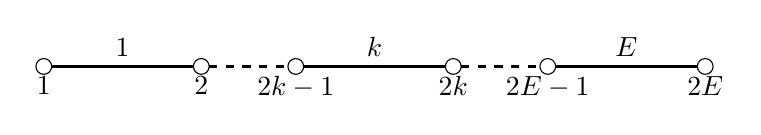
\begin{tikzpicture}
  \draw (2.3,0) circle (0.1) node [below] {$1$};
  \draw (4.3,0) circle (0.1) node [below] {$2$};
  \draw[thick] (2.4,0) -- (4.2,0) node [above,midway] {$1$};
  \draw[thick,dashed] (4.4,0) -- (5.4,0);
  \draw (5.5,0) circle (0.1) node [below] {$2k-1$};
  \draw (7.5,0) circle (0.1) node [below] {$2k$};
  \draw[thick] (5.6,0) -- (7.4,0) node [above,midway] {$k$};
  \draw[thick,dashed] (7.6,0) -- (8.6,0);
  \draw (8.7,0) circle (0.1) node [below] {$2E-1$};
  \draw (10.7,0) circle (0.1) node [below] {$2E$};
  \draw[thick] (8.8,0) -- (10.6,0) node [above,midway] {$E$};
\end{tikzpicture}

  \caption{One-dimensional mesh made of $E$ elements of constant length $\Delta X = \frac{l}{E}$.}\label{fig:1Dmesh}
\end{figure}

Since fields are carried by particles, we seek for the scheme equation that gives the solution $\bar{Q}$ at a material point for a given time step, with respect to the solutions of other particles at previous time step. In this section, lower and case symbols are respectively devoted to nodes and material points. Furthermore, since we consider here scalar quantities, the information on nodes and particles can be written as subscripts without ambiguity. Hence, at the time step $n$, the solution at material point $I$ reads $Q^{n}_I$ and it is the same for nodes. Then, the cell containing a given particle $J$ will be denoted by $c(J)$ so that the nodes interacting with this particle are $2c(J)-1$ and $2c(J)$. At last, the linear shape functions defined in element $c(J)$ are:
\begin{equation}
S_{2c(J)-1}(X)= \frac{X^{2c(J)} - X}{\Delta X} \qquad S_{2c(J)}(X)= \frac{X -X^{2c(J)-1}}{\Delta X} \qquad X \in \[X^{2c(J)-1},X^{2c(J)}\]
\end{equation}
and $S_{i,J}$ is the shape function of node $i$ evaluated at the position of the $I$th material point.

\subsubsection*{DGMPM scheme equation}
\label{subsec:scheme_Euler}
The method followed to write the scheme equation is to trace backward the numerical procedure described in section \ref{sec:DGMPM} in order to get an expression of the form \eqref{eq:general_scheme} for the material point $I$:
\begin{equation}
\bar{Q}^{n+1}_I = H\(\bar{Q}^{n}_K\) \qquad  K=1,..,N_p
\end{equation} 
Quantities at time $t^{n+1}$ are obtained by interpolating nodal solutions of the discrete equation \eqref{eq:DGMPM_discrete} in the cell containing the $I$th particle by the projection \eqref{eq:DGMPM_node2points}: 
\begin{equation}
\bar{Q}^{n+1}_I = S_{2c(I)-1,I}\bar{q}_{2c(I)-1}^{n+1} + S_{2c(I),I}\bar{q}_{2c(I)}^{n+1} \label{eq:updated_MP}
\end{equation}
With the interface fluxes in the case of the linear scalar advection equation $\Fc_N =  (aq^*) N $, in which $q^*$ is the stationary solution of Riemann's problem at the cell interface and $N=\pm 1$ the outward unit normal, the discrete form \eqref{eq:DGMPM_discrete} leads to the following expressions of updated nodal values:
\begin{equation}
  \label{eq:nodal_discrete_forms}
  \begin{aligned}
    & \bar{q}_{2c(I)-1}^{n+1}= \bar{q}_{2c(I)-1}^{n} + \frac{\Delta t}{M^L_{2c(I)-1}}\( K_{2c(I)-1,j} a\bar{q}_{j}^{n}- a\rho \bar{q}_{2c(I)-1}^*N_{2c(I)-1} \)\\
    &\bar{q}_{2c(I)}^{n+1}= \bar{q}_{2c(I)}^{n} + \frac{\Delta t}{M^L_{2c(I)}}\( K_{2c(I),j} a\bar{q}_{j}^{n}- a\rho \bar{q}_{2c(I)}^*N_{2c(I)} \)
  \end{aligned}
\end{equation}
Equations \eqref{eq:nodal_discrete_forms} can be simplified by first noting that in a one-dimensional grid, the outward unit vectors are $N_{2c(I)-1}=-1$ and $N_{2c(I)}=1$. Then, provided linear shape functions, the lumped mass and the pseudo-stiffness matrices are:
\begin{align}
  & M^L_i = \sum_{J=1}^{N_p} S_{iJ} m_J \\
  & K_{2c(I)-1,j} = \sum_{J=1}^{N_p} \drond{S_{2c(I)-1,J}}{X} m_J S_{jJ} = -\sum_{J=1}^{N_p} \frac{m_J S_{jJ}}{\Delta X} \\
  & K_{2c(I),j} = \sum_{J=1}^{N_p} \drond{S_{2c(I),J}}{X} m_J S_{jJ} = \sum_{J=1}^{N_p} \frac{m_J S_{jJ}}{\Delta X} 
\end{align}
where $m_J$ is the mass of $J$th material point. The discontinuous approximation basis moreover yields a bloc diagonal pseudo-stiffness matrix so that one can write:
\begin{equation}
  \label{eq:block_diag_K}
  K_{i,j} \bar{q}_{j}^{n}= K_{i,2c(i)-1} \bar{q}_{2c(i)-1}^{n}+K_{i,2c(i)} \bar{q}_{2c(i)}^{n}
\end{equation}
Furthermore, in a homogeneous medium the mass density can be replaced by $\rho = N_p^{c( I)} m_I/\Delta X$ where $N_p^{c( I)}$ is the number of particles in the cell that contains the $I$th material point. Since waves travel from left to right ($a>0$), the stationary solution is equal to the value at the upwind node of an interface, that is:
\begin{align}
  & q_{2c(I)-1}^* = \rho \bar{q}^n_{2c(I)-2}=  N_p^{c( I)}\frac{ m_I}{\Delta X}\bar{q}^n_{2c(I)-2} \\
  & q_{2c(I)}^* = \rho \bar{q}^n_{2c(I)} =  N_p^{c( I)}\frac{ m_I}{\Delta X} \bar{q}^n_{2c(I)} 
\end{align}

Gathering all the previous consideration and seeing that the definition of the mass density used implies that every particles in a given cell carry the same mass, equations \eqref{eq:nodal_discrete_forms} read:
\begin{equation}
  \label{eq:nodal_discrete_forms_simplified}
  \begin{aligned}
    & \bar{q}_{2c(I)-1}^{n+1}= \bar{q}_{2c(I)-1}^{n} - \frac{a\Delta t}{\Delta X}\( \frac{\sum_{L=1}^{N_p^{c(I)}} \[S_{2c(I)-1,L}\bar{q}_{2c(I)-1}^{n}+ S_{2c(I),L}\bar{q}_{2c(I)}^{n}\] - N_p^{c( I)} \bar{q}^n_{2c(I)-2}}{\sum_{J=1}^{N_p^{c(I)}}  S_{2c(I)-1,J}}\)\\
    &\bar{q}_{2c(I)}^{n+1}= \bar{q}_{2c(I)}^{n} + \frac{a\Delta t}{\Delta X}\( \frac{\sum_{L=1}^{N_p^{c(I)}}\[S_{2c(I)-1,L}\bar{q}_{2c(I)-1}^{n}+ S_{2c(I),L}\bar{q}_{2c(I)}^{n}\]- N_p^{c( I)}  \bar{q}^n_{2c(I)}}{\sum_{J=1}^{N_p^{c(I)}}  S_{2c(I),J}} \)
  \end{aligned}
\end{equation}
where the Courant number $CFL=a\Delta t/\Delta X$ arises. Introduction of those equation in the updated material point solution \eqref{eq:updated_MP} leads after some simplifications to:
\begin{equation}
  \begin{split}
    \bar{Q}^{n+1}_I =  &\(S_{2c(I)-1,I} - \frac{a\Delta t}{\Delta X}\sum_{L} S_{2c(I)-1,L}\[\frac{S_{2c(I)-1,I}}{\sum_{J}  S_{2c(I)-1,J}} - \frac{S_{2c(I),I}}{\sum_{J}  S_{2c(I),J}}\] \)\bar{q}_{2c(I)-1}^{n} \\+&\( S_{2c(I),I}+\frac{a\Delta t}{\Delta X}\sum_{L} S_{2c(I),L}\[\frac{S_{2c(I),I}}{\sum_{J}  S_{2c(I),J}} - \frac{S_{2c(I)-1,I}}{\sum_{J}  S_{2c(I)-1,J}}\] - N_p^{c(I)}\frac{a\Delta t}{\Delta X}\frac{S_{2c(I),I}}{\sum_{J}  S_{2c(I),J}}\)\bar{q}_{2c(I)}^{n}\\
    + &N_p^{c(I)}\frac{a\Delta t}{\Delta X}\frac{S_{2c(I)-1,I}}{\sum_{J}  S_{2c(I)-1,J}}\bar{q}_{2c(I)-2}^{n}
  \end{split}
\end{equation}
\begin{equation}
  \label{eq:euler_before_mapping}
  \begin{split}
    \bar{Q}^{n+1}_I =  &\(S_{2c(I)-1,I} - \frac{a\Delta t}{\Delta X}\[S_{2c(I)-1,I} - \frac{S_{2c(I),I}\sum_{L} S_{2c(I)-1,L}}{\sum_{J}  S_{2c(I),J}}\] \)\bar{q}_{2c(I)-1}^{n} \\+&\( S_{2c(I),I}+\frac{a\Delta t}{\Delta X}\[S_{2c(I),I} - \frac{S_{2c(I)-1,I}\sum_{L} S_{2c(I),L}}{\sum_{J}  S_{2c(I)-1,J}}\] - N_p^{c(I)}\frac{a\Delta t}{\Delta X}\frac{S_{2c(I),I}}{\sum_{J}  S_{2c(I),J}}\)\bar{q}_{2c(I)}^{n}\\
    + &N_p^{c(I)}\frac{a\Delta t}{\Delta X}\frac{S_{2c(I)-1,I}}{\sum_{J}  S_{2c(I)-1,J}}\bar{q}_{2c(I)-2}^{n}
  \end{split} 
\end{equation}

In equation \eqref{eq:euler_before_mapping} the solutions at nodes result from the convection step \eqref{eq:DGMPM_points2nodes}:
\begin{equation}
\bar{q}^{n}_{i} = \frac{\sum_K S_{iK}m_K \bar{Q}^n_{K}}{\sum_P S_{iP}m_P} = \frac{\sum_K S_{iK} \bar{Q}^n_{K}}{\sum_P S_{iP}} \label{eq:stab_mapping}
\end{equation}
Thus, introduction of mapping \eqref{eq:stab_mapping} in equation \eqref{eq:euler_before_mapping} and permutation of sums over $K$ and $i$ lead after some simplifications to the scheme equation:
\begin{equation}
  \begin{split}
    \bar{Q}^{n+1}_I = \sum_{K=1}^{N_p} \bar{Q}^{n}_K &S_{2c(I)-1,K}\(\frac{S_{2c(I)-1,I}}{\sum_P S_{2c(I)-1,P}} - \frac{a\Delta t}{\Delta X}\[\frac{S_{2c(I)-1,I}}{\sum_P S_{2c(I)-1,P}} - \frac{S_{2c(I),I}}{\sum_{J}  S_{2c(I),J}}\] \) \\
  +\sum_{K=1}^{N_p} \bar{Q}^{n}_K&S_{2c(I),K}\( \frac{S_{2c(I),I}}{\sum_P S_{2c(I),P}}+\frac{a\Delta t}{\Delta X}\[\frac{S_{2c(I),I}}{\sum_P S_{2c(I),P}} - \frac{S_{2c(I)-1,I}}{\sum_{J}  S_{2c(I)-1,J}}\] - N_p^{c(I)}\frac{a\Delta t}{\Delta X}\frac{S_{2c(I),I}}{\(\sum_{J}  S_{2c(I),J}\)^2}\)\\
    + \sum_{K=1}^{N_p} \bar{Q}^{n}_K &S_{2c(I)-2,K}N_p^{c(I)}\frac{a\Delta t}{\Delta X}\frac{S_{2c(I)-1,I}}{\sum_{J}  S_{2c(I)-1,J}\sum_{P}  S_{2c(I)-2,P}}
  \end{split}
\end{equation}
\begin{equation}
  \begin{split}
    \bar{Q}^{n+1}_I = \sum_{K=1}^{N_p} \bar{Q}^{n}_K  &\(\overbrace{\sum_{i=1}^{2E}S_{iK}\frac{S_{iI}}{\sum_P S_{iP}}}^{A} - \frac{a\Delta t}{\Delta X} \overbrace{\(S_{2c(I)-1,K}+S_{2c(I),K}\)\[\frac{S_{2c(I)-1,I}}{\sum_P S_{2c(I)-1,P}} - \frac{S_{2c(I),I}}{\sum_{J}  S_{2c(I),J}}\]}^{B} \right.\\
    & + \left.  N_p^{c(I)}\frac{a\Delta t}{\Delta X} \underbrace{\[\frac{S_{2c(I)-2,K}}{\sum_{P}  S_{2c(I)-2,P}}\frac{S_{2c(I)-1,I}}{\sum_{J}  S_{2c(I)-1,J}}-\frac{S_{2c(I),I}}{\sum_{J}  S_{2c(I),J}}\frac{S_{2c(I),K}}{\sum_{J}  S_{2c(I),J}}\]}_{C} \vphantom{\sum_{i=1}^{2E}}\)
  \end{split}
\end{equation}
Only one cell is covered by the support of the shape functions so that the only non-vanishing terms in term $A$ are those involving the nodes of cells $c(K)$ and $c(I)$ if particles $K$ and $I$ share the same element. On the other hand, the parenthesis in $B$ is unity if $c(I)=c(K)$ and zero otherwise, so that:
\begin{equation*}
  B= \[\frac{S_{2c(K)-1,I}}{\sum_P S_{2c(K)-1,P}} - \frac{S_{2c(K),I}}{\sum_{J}  S_{2c(K),J}}\]
\end{equation*}
At last, the first term in $C$ is not zero if $K$ is contained in cell upwind cell of that of $I$ while the second one does not vanish for $K$ and $I$ sharing the same element. Hence, the final expression of the scheme equation for the scalar linear advection equation is:
\begin{equation}
  \label{eq:Euler_scheme}
  \begin{split}
    \bar{Q}^{n+1}_I = \sum_{K=1}^{N_p} \bar{Q}^{n}_K  &\left\lbrace\sum_{i=1}^{2E}S_{iK}\frac{S_{iI}}{\sum_P S_{iP}} - \frac{a\Delta t}{\Delta X} \[\frac{S_{2c(K)-1,I}}{\sum_P S_{2c(K)-1,P}} - \frac{S_{2c(K),I}}{\sum_{J}  S_{2c(K),J}}\] \right.\\
    & + \left.  N_p^{c(I)}\frac{a\Delta t}{\Delta X} \[\frac{S_{2c(K),K}}{\sum_{P}  S_{2c(K),P}}\frac{S_{2c(K)+1,I}}{\sum_{J}  S_{2c(K)+1,J}}-\frac{S_{2c(K),I}}{\sum_{J}  S_{2c(K),J}}\frac{S_{2c(K),K}}{\sum_{J}  S_{2c(K),J}}\] \vphantom{\sum_{i=1}^{2E}}\right\rbrace
  \end{split}
\end{equation}

In a similar way, the two-stage RK2 time integration leads to the following scheme equations (see Appendix \ref{sec:RK2_scheme} for details):
\begin{equation}
  \label{eq:RK2_scheme}
  \begin{split}
    \bar{Q}^{n+1}_I =  \sum_{K} Q_K^n  & \left\lbrace \frac{S_{2c(I)-1,I}}{\sum_{J}  S_{2c(I)-1,J}}\(S_{2c(I)-1,K}-\frac{a\Delta t}{\Delta X} + \frac{1}{2}\(\frac{a\Delta t}{\Delta X}\)^2N_p^{c(I)}\frac{S_{2c(I),K} }{\sum_{J}  S_{2c(I),J}}\) \right. \\
    + \frac{S_{2c(I),I}}{\sum_{J}  S_{2c(I),J}}&\(S_{2c(I),K} + \frac{a\Delta t}{\Delta X}\[1-N_p^{c(I)}\frac{S_{2c(I),K}}{\sum_{J}  S_{2c(I),J}}\] - \frac{N_p^{c(I)}\(\frac{a\Delta t}{\Delta X}\)^2}{2\sum_{J}  S_{2c(I),J}}\[1+S_{2c(I),K}-\frac{N_p^{c(I)}S_{2c(I),K}}{\sum_{J}  S_{2c(I),J}}\]\)\\
     + \frac{S_{2c(I)-2,K}}{\sum_{J}  S_{2c(I)-2,J}}&\left.\frac{a\Delta t}{\Delta X}N_p^{c(I)}\( \frac{S_{2c(I)-1,I}}{\sum_{L}  S_{2c(I)-1,L}}\[1-\frac{a\Delta t}{2\Delta X}\(\frac{N_p^{c(I)-1}}{\sum_{L}  S_{2c(I)-2,L}}+1\)\] + \frac{a\Delta t}{2\Delta X}\frac{S_{2c(I),I}}{\sum_{L}  S_{2c(I),L}}\)\right\rbrace
   \end{split}
\end{equation}
\begin{equation}
  \label{eq:RK2_scheme}
  \begin{split}
    \bar{Q}^{n+1}_I =  \sum_{K} Q_K^n   &\left\lbrace \sum_{i=1}^{2E}S_{iK}\frac{S_{iI}}{\sum_P S_{iP}} - \frac{a\Delta t}{\Delta X} \[\frac{S_{2c(K)-1,I}}{\sum_P S_{2c(K)-1,P}} - \frac{S_{2c(K),I}}{\sum_{J}  S_{2c(K),J}}\] \right.\\   & \frac{S_{2c(I)-1,I}}{\sum_{J}  S_{2c(I)-1,J}}\( + \frac{1}{2}\(\frac{a\Delta t}{\Delta X}\)^2N_p^{c(I)}\frac{S_{2c(I),K} }{\sum_{J}  S_{2c(I),J}}\)  \\
    %%%
    & adding
    %%%
    \\
    + \frac{S_{2c(I),I}}{\sum_{J}  S_{2c(I),J}}&\( - \frac{a\Delta t}{\Delta X}N_p^{c(I)}\frac{S_{2c(I),K}}{\sum_{J}  S_{2c(I),J}} - \frac{N_p^{c(I)}\(\frac{a\Delta t}{\Delta X}\)^2}{2\sum_{J}  S_{2c(I),J}}\[1+S_{2c(I),K}-\frac{N_p^{c(I)}S_{2c(I),K}}{\sum_{J}  S_{2c(I),J}}\]\)\\
     + \frac{S_{2c(I)-2,K}}{\sum_{J}  S_{2c(I)-2,J}}&\left.\frac{a\Delta t}{\Delta X}N_p^{c(I)}\( \frac{S_{2c(I)-1,I}}{\sum_{L}  S_{2c(I)-1,L}}\[1-\frac{a\Delta t}{2\Delta X}\(\frac{N_p^{c(I)-1}}{\sum_{L}  S_{2c(I)-2,L}}+1\)\] + \frac{a\Delta t}{2\Delta X}\frac{S_{2c(I),I}}{\sum_{L}  S_{2c(I),L}}\)\right\rbrace
   \end{split}
\end{equation}
which can be written for simplicity:
\begin{equation}
\bar{Q}^{n+1}_I = \sum_{K=1}^{N_p} \bar{Q}^n_{K} D_{IK} \label{eq:scheme_Dpi}
\end{equation}



The numerical solution $\bar{Q}^{n+1}_I$ depends on the Courant number $a\Delta t / \Delta X$ and on the position of material points within the grid mesh through the shape functions in the expression of coefficients $D_{IK}$. Furthermore, the first (\textit{resp. second}) brackets in equation \eqref{eq:Dalpha_mu} involve shape functions that are non zero if material point $K$ and $I$ lie in the same cell (\textit{resp. previous cell}). This property means that the numerical domain of dependence of the DGMPM for scalar linear advection with $a>0$ covers two cells regardless of the number of material points. If one looks at the particular case of one material point lying in every cell, then il comes: 

\subsubsection*{2D Euler CTU}

\subsubsection*{The von Neumann linear stability analysis}
The computational domain is now repeated periodically by mapping it to the domain $[-l,0]$ so that the solution at material point $J$ and time step $n$ is expanded into a discrete Fourier basis of $2E+1$ harmonics over the domain $X \in \[-l,l\]$:
\begin{equation}
\bar{Q}^{n}_J = \sum_{j=-E}^{E}A_j^n e^{I J k_j \Delta X}
\end{equation}
with $A^n_j$, the magnitude of the $j$th harmonic at time step $n$, $I = \sqrt{-1}$, and $k_j$ a wave number. Introduction of this expansion in equation \eqref{eq:scheme_Dpi} yields:
\begin{equation}
A_j^{n+1} e^{I I k_j \Delta X} = \sum_{K=1}^{N_p} A_j^n D_{IK}e^{I K k_j \Delta X}\quad \forall j=-E,...,E
\end{equation}
The amplification factor between two time steps at a given point is defined as:
\begin{equation}
\frac{A_j^{n+1}}{A_j^n} = \sum_{K=1}^{N_p} e^{I (K -I)k_j \Delta X} D_{IK} \quad \forall j=-E,...,E \label{eq:fourier}
\end{equation}
A necessary condition to ensure the stability of a numerical scheme is that the amplification factor must be lower than one in modulus: $\abs{A^{n+1}/A^n} < 1$. This upper bound allows to ensure that eventual errors do not increase during the computation. For expression \eqref{eq:fourier}, this leads to:
\begin{equation}
 \abs{\sum_{K=1}^{N_p} e^{I (K -I)k_j \Delta X} D_{IK}} \leq \sum_{K=1}^{N_p} \abs{e^{I (K -I)k_j \Delta X} D_{IK}} = \sum_{K=1}^{N_p} \abs{D_{IK}}
\end{equation}
where the triangle inequality, and the unit modulus of the complex number $e^{I (K -I)k_j \Delta X}$ have been used.
Hence, the DGMPM scheme is stable for a given discretization if the Courant number is set so that the following condition is satisfied:
\begin{equation}
\sum_{K=1}^{N_p} \abs{D_{IK}} \leq 1 \label{eq:stability}
\end{equation}
According to the scheme equation \eqref{eq:Dalpha_mu}, such a stability condition can be very hard to deal with analytically for general discretizations. However, the particular configuration for which one single particle lies in each cell can be studied analytically. In this case, condition \eqref{eq:stability} reads:
\begin{equation}
\sum_{K=1}^{N_p} \abs{D_{IK}} = \abs{1 - a\frac{\Delta t}{\Delta X} } +  \abs{ a\frac{\Delta t}{\Delta X} } \leq 1 \label{eq:1ppc_stab}
\end{equation}
which is satisfied for all $a\frac{\Delta t}{\Delta X} \leq 1$ regardless of the positions of particles.
Hence, this space discretization leads to a stable scheme for the optimal Courant condition while the classical DGFEM scheme developed in \cite{Chavent_Salzano} is restricted to condition $\Delta t / \Delta X = \Oc(\sqrt{\Delta X})$. Recall that this DGMPM space discretization can be viewed as a DGFEM with reduced integration of the weak form (see section \ref{section:discretization}). Hence, combination of reduced integration with projections between mesh nodes and integration points allows to improve the restrictive stability condition of original DGFEM \cite{Chavent_Salzano,NeutronDG}. However, this optimal condition is no longer valid for discretizations involving more than one material point per cell. Indeed, figure \ref{figure:Amplification_factor} shows the evolution of the amplification factor with respect to the Courant number for several (regular) discretizations. Since the scheme equation \eqref{Dalpha_mu} depends on the particle considered, those curves are plotted for each material point contained in a given cell. In figures \ref{figure:Amplification_factor}\subref{subfig:CFL_2ppc} and \ref{figure:Amplification_factor}\subref{subfig:CFL_3ppc} we can see that the amplification factor satisfies the stability condition \eqref{stability} for CFL numbers lower than one.

%%% Table of CFL that can be reached depending on the discretization
Two material points in each cell are considered in figure \ref{figure:Amplification_factor}\subref{subfig:CFL_2ppc}, with either a symmetrical or an offset configuration, respectively shown in figures \ref{figure:Amplification_factor}\subref{subfig:conf1} and \ref{figure:Amplification_factor}\subref{subfig:conf2}. It also appears that the more restrictive condition on CFL number is given by the upwind (first) material point ($CFL=0.43$ for symmetrical configuration and $CFL=0.34$ for shifted one). Moreover, the material points positions influence the stability condition as shown by the shifted configuration for which the result is more restrictive. Similar observations can be made with figure \ref{figure:Amplification_factor}\subref{subfig:CFL_3ppc} in which three particles are considered. In that case, Courant number decreases to $CFL=0.29$ for configuration \ref{figure:Amplification_factor}\subref{subfig:conf3} and $CFL=0.26$ for configuration \ref{figure:Amplification_factor}\subref{subfig:conf4}. 

The von Neumann linear stability analysis performed in this section provides an explicit (nonlinear) condition \eqref{stability} that must be satisfied in order to ensure the stability of the DGMPM scheme. First, this relation allows to fully exploit the ability of the method to rebuild the grid mesh arbitrarily. Indeed, after such a procedure, the number and positions of material points in grid cells can change and one must be able to adapt properly the CFL number in order to ensure stability. An advantage on the original MPM is hence highlighted since no stability condition exists for the latter scheme. Second, it has been shown that some DGMPM discretizations provide an improvement of the restrictive CFL number that applies to the DGFEM scheme. In particular, the optimal condition allowing to capture discontinuities ($CFL=1$) can be reached when one particle lies in each cell of the grid mesh. This property turns out to be a strength for the DGMPM since it aims at follow waves accurately as shown with the following numerical results.


+ RK2 ??
\subsection{Two-dimensional stability analysis}


\subsection{Non-linear stability analysis}
Convergence to entropy solution ; Non-linear stability ; entropy inequality
see \cite[p.219]{Leveque}, where lax entropy condition may be used instead of such an entropy inequality

Convergence in linear case is just mentioned and not shown in \cite{Cockburn}. But for non-linear cases it is based on the entropy inequality.

%% Test diffusion with limiters influence in the test case riemann_prob.py in DGMPM/elasticity
\subsection{Convergence analysis}
see Roe theorem \cite[p.417]{Toro}


Pfffff, franchement on peut en parler mais c'est bien relou à interpréter tellement ça dépend de la discretisation. On peut par exemple montrer qu'on est monotone pour 1ppc (FOU method) donc ordre 1. On peut aussi dire que ce n'est pas évident pour 2ppc. Après avoir dit ça, tracer des courbes de convergences paraît futile. Donc ça implique de développer la scheme equation, faire la stabiliter pour bien buter tout le monde et finir par la convergence.

%%% Local Variables: 
%%% mode: latex
%%% TeX-master: "../mainManuscript"
%%% End:
